\section{Einlesen}
\subsection{\fbox{read\_csv - read\_csv2}}
\textbf{Erzeugt Tibble}\\
\textbf{read\_csv}: Komma zum Zeilentrennen und Punkt für Dezimalzahlen\\
\textbf{read\_csv2}: Semicolon zum Zeilentrennen und Komma für Dezimalzahlen
\begin{rcode}{1]}
read_csv(file = "", col_types = "")
read_csv2(file = "", col_types = "")
\end{rcode}
Mit col\_types können wir als String wo jede Position für die jeweilige Spalten steht den Typ bestimmen\\
\textbf{Typen:}
\begin{itemize}[noitemsep]
  \item \textbf{c} = character
  \item \textbf{i} = integer
  \item \textbf{n} = number
  \item \textbf{d} = double
  \item \textbf{l} = logical
  \item \textbf{f} = factor
  \item \textbf{D} = date
  \item \textbf{T} = date time
  \item \textbf{t} = time
  \item \textbf{?} = guess
  \item \textbf{\_ oder -} = skip
\end{itemize}
\begin{rcode}{1]}
# Csv with ";" separator and "." as decimal point
read.csv("europe.data.csv", sep = ";", dec=".")

# Csv without first line as header
read.csv2("mpg.csv", header=F)

# Csv with 4 integer columns
read_csv2("magnets_pain.csv", 
            col_types = "iiii")
\end{rcode}
\subsection{\fbox{read.csv - read.csv2}}
\textbf{Erzeugt Dataframe}
\begin{rcode}{1]}
data <- read.csv(file="", sep = ";", dec = ".") %>% as_tibble()
\end{rcode}
\begin{itemize}[noitemsep]
  \item \textbf{sep} = Das Zeichen welches die Spalten trennt.
  \item \textbf{dec} = Gibt den trenner für Dezimalzahlen an
\end{itemize}
\subsection{\fbox{read\_delim - read\_delim2}}
\textbf{Erzeugt Tibble}\\
Der Rest wie bei \_
\begin{rcode}{1]}
read_delim(file = , delim = ,col_types = "")
\end{rcode}
Mit der Option \textbf{delim} können wir festlegen, mit welchem Zeichen die Zeilen getrennt werden. 
\columnbreak
\subsection{\fbox{Tidy Data}}
\textbf{Typen:}
\begin{itemize}[noitemsep]
  \item Jede Spalte muss eine Variable sein,
  \item Eine Observation ist eine Zeile,
  \item Eine Variable ist Z.b das Alter,
  \item Die einzelnen Daten sind die Beobachtungen
\end{itemize}

\normalsize
\section{\fbox{Tidying Data}}
\subsection{\fbox{pivot\_longer()}}
\textbf{Wir haben eine Tabelle wo es Spalten gibt die als Variablen selber Observationen haben. Wir wollen diese Observationen auch als Observationen hinschreiben}\\

\frame{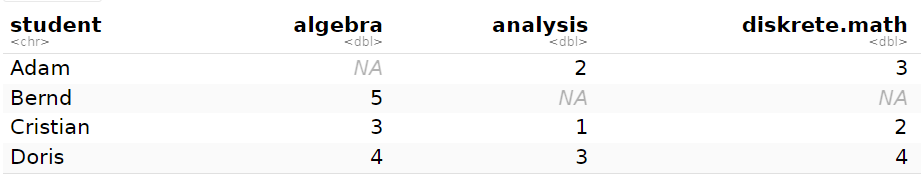
\includegraphics[draft=false, width=1\linewidth]{Figures/pivotlonger.png}}
Wir sehen, dass algebra etc eigentlich Observations sind.
\begin{rcode}{1]}
student1 %>% pivot_longer(cols =          algebra:diskrete.math, names_to = "classes", values_to = "grade", values_drop_na = T)
\end{rcode}
\begin{itemize}[noitemsep]
  \item \textbf{cols} = ein c() mit allen spalten oder spalte\_1 : spalte\_n.,
  \item \textbf{names\_to} = In welche Spalte die Namens aus cols.,
  \item \textbf{values\_to} = In Welche Spalte die Werte die in den Spalten aus cols waren,
  \item \textbf{values\_drop\_na} = T falls wir NAs droppen wollen
\end{itemize}
\frame{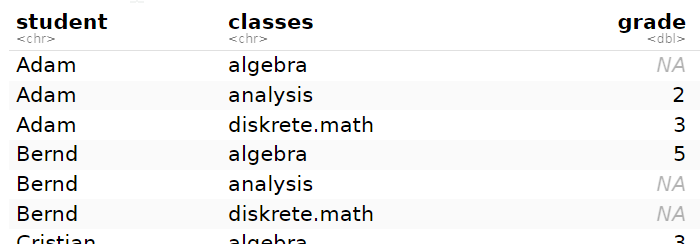
\includegraphics[draft=false, width=1\linewidth]{pivotlonger2.png}}
Hier haben wir jetzt in jeder Spalte eine Variable
\subsection{\fbox{pivot\_longer}}
Wir haben in einer Spalte für jede Observation zwei Variablen und in einer anderen Spalte die Observation für jede Variable
\frame{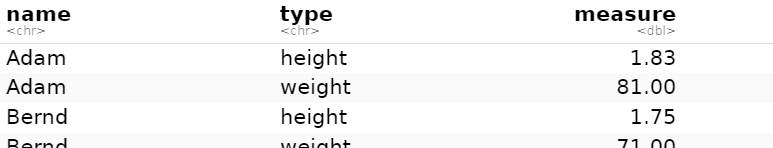
\includegraphics[draft=false, width=1\linewidth]{pivotwider.png}}
Jede Variable in Type soll eine eigene Spalte bekommen
\begin{rcode}{1]}
student2 %>% pivot_wider(names_from = type, values_from = measure)
\end{rcode}
\begin{itemize}[noitemsep]
  \item \textbf{names\_from} = Die Spalte in der die Variablen stehen.,
  \item \textbf{values\_from} = Die Spalte wo die Observationen drinne stehen.
\end{itemize}
\frame{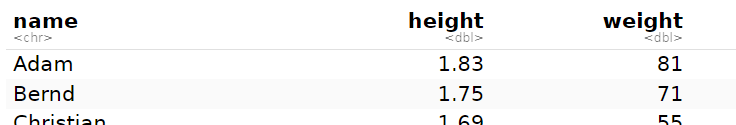
\includegraphics[draft=false, width=1\linewidth]{Figures/pivotwider2.png}}
Jetzt hat jede Variable eine Spalte
\newpage
\section{\fbox{separate}}
Wir haben in einer Spalte Zwei Observations in einer Zelle
\frame{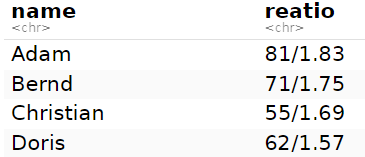
\includegraphics[draft=false, width=1\linewidth]{Figures/seperate.png}}
Nun wollen wir diese Spalte aufteilen


\begin{rcode}{1}
student3 %>% separate(col = reatio, sep = "/", into = c("weight", " height"))
\end{rcode}
\begin{itemize}[noitemsep]
  \item \textbf{col} = Die Spalte in der die Observations sind.
  \item \textbf{sep} = Das Zeichen, welches die Observations trennt.
  \item \textbf{into} = Ein Array in welches die Observations nun geschrieben werden sollen.
\end{itemize}
\frame{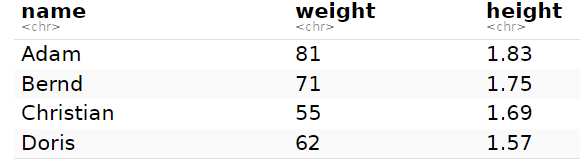
\includegraphics[draft=false, width=1\linewidth]{Figures/separate2.png}}
\begin{comment}
\begin{markdown}
# Wichtige Befehle
## Librarys
```R
library(tidyverse)
library(TeachingDemos)
```

## Datenerzeugung
- **sample** = Erzeugt ein sample aus den Werten in dem Array x mit der Länge size. Replace auf True wenn wir nur Unique werte aus x wollen.
- **runif** = Ein array mit länge n mit werten von min bis max

```R
students <- tibble(
  id = 1:10,
  sex = sample(x = c("f", "m"), size = 10, replace = T),
  age = round(runif(n = 20, min = 10, max = 35)),
)
```

\end{markdown}

\end{comment}
